\documentclass{easychair}

\usepackage{doc}

\newcommand{\easychair}{\textsf{easychair}}
\newcommand{\miktex}{MiK{\TeX}}
\newcommand{\texniccenter}{{\TeX}nicCenter}
\newcommand{\makefile}{\texttt{Makefile}}
\newcommand{\latexeditor}{LEd}

\usepackage{graphicx}
\graphicspath{ {./images/} }
\usepackage{float}

\usepackage{listings}
\usepackage{xcolor}

\usepackage{tcolorbox}

\definecolor{gray}{RGB}{242, 242, 242}
\definecolor{black}{RGB}{0,0,0}
\definecolor{commentstyle}{RGB}{157, 158, 15}
\definecolor{keywordstyle}{RGB}{156, 4, 17}
\definecolor{stringstyle}{RGB}{4, 156, 7}
\definecolor{darkviolet}{rgb}{0.58, 0.0, 0.83}
\definecolor{royalblue}{rgb}{0.25, 0.41, 0.88}
\definecolor{crimson}{rgb}{0.86, 0.8, 0.24}

\lstdefinestyle{myStyle}{
    backgroundcolor=\color{gray},   
    commentstyle=\color{commentstyle},
    keywordstyle=\color{keywordstyle},
    stringstyle=\color{stringstyle},
    numberstyle=\tiny\color{black},
    emphstyle=\color{crimson},
    basicstyle=\ttfamily\color{black}\scriptsize,
    frame=leftline,
    rulecolor=\color{black},
    breakatwhitespace=false,  
    captionpos=b,
    breaklines=true,                 
    captionpos=b,                    
    keepspaces=true,                 
    numbers=left,                    
    numbersep=7pt,   
    xleftmargin=3.5ex,
    showspaces=false,                
    showstringspaces=false,
    showtabs=false,                  
    tabsize=2,
    extendedchars=true,  % requires inputenc
  fontadjust=true,
  keywordstyle={[2]\color{darkviolet}},
  keywordstyle={[3]\color{royalblue}},
  upquote=true  % requires textcomp
}


\lstset{style=myStyle}

\lstdefinelanguage{JavaScript}{
  morekeywords=[1]{break, readonly, continue, delete, else, for, if, in,
    new, return, this, typeof, var, void, while, with, const, Blob, <T>},
  % Literals, primitive types, and reference types.
  morekeywords=[2]{false, null, true, boolean, number, undefined,
    Array, Boolean, Date, Math, Number, String, Object, string,T, <T> },
  % Built-ins.
  morekeywords=[3]{await, async, case, catch, class,interface, function, default, do,
    enum, export, extends, finally, from, implements, import, instanceof,
    let, static, super, switch, throw, try, public},
    morekeywords=[4]{}, 
    sensitive,
  morecomment=[s]{/*}{*/},
  morecomment=[l]//,
  morecomment=[s]{/**}{*/}, % JavaDoc style comments
  morestring=[b]',
  morestring=[b]`,
  morestring=[b]",
}[keywords, comments, strings]

\usepackage[ngerman]{babel}

\title{Das Expression Problem: Lösung mit Generics in TS\footnote{TS: TypeScript}
\thanks{Der vorliegende Titel basiert auf Mads Torgersens Papier „The Expression Problem Revisited“. Es behandelt Definitionen und Konzepte zur Lösung und Implementierung in TypeScript für den Proseminar-Kurs.}}

\author{Mohammadreza Javadikouchaksaraei}

\institute{
  Technische Universität Dortmund\\
  Informatik Student mit Matrikelnummer 234019\\
  \email{mohammadreza.javadikouchaksaraei@tu-dortmund.de}
}

\authorrunning{M. Javadikouchaksaraei: 234019}

\titlerunning{Das Expression Problem: Lösung mit Generics in TS}

\begin{document}

\maketitle

\setcounter{tocdepth}{2}
{\small
\tableofcontents}

\newpage

\section{Einleitung}
Das „Expression Problem“ stellt seit jeher eine Herausforderung im Design von Programmiersprachen dar, die die Gestaltung und Implementierung objektorientierter und funktionaler Sprachen maßgeblich beeinflusst. Das Ziel besteht in der Definition eines Datentyps, welcher die Hinzufügung neuer Fälle zum Datentyp sowie die Implementierung neuer Funktionen über den Datentyp ohne erneute Kompilierung des Codes ermöglicht, während gleichzeitig die statische Typensicherheit bewahrt wird \cite{wadler1998expression}. Es gibt verschiedene Ansätze zur Lösung dieses Problems, die jeweils ihre eigenen Vor- und Nachteile haben.\\

In dieser Ausarbeitung für den Proseminarkurs wurden klassische und moderne Methoden zur Lösung des \textit{Expression Problems} mit \textit{Generics} analysiert, basierend auf dem Artikel „The Expression Problem Revisited: Four new solutions using generics“ \cite{torgersen2004expression}. Das Ziel ist es, dieses Ansatz in TypeScript zu implementieren und zu testen.

\section{Grundlagen des Expression Problems}
  \subsection{Beschreibung des Expression Problems}
  \subsubsection{Historie}
Um die Genese des vorliegenden Problems zu verstehen, ist ein Blick auf die Arbeit von John Reynolds aus dem Jahr 1975 erforderlich. Reynolds identifizierte das Problem in seinen Untersuchungen zur Datenverwaltung in der Programmierung und präsentierte zwei Ansätze: benutzerdefinierte Typen (ADTs\footnote{ADTs: Abstrakte Datentypen, eine Methode, bei der alle Informationen zur Datenrepräsentation zentral zusammengefasst werden.}) und prozedurale Datenstrukturen \cite{Reynolds1978}. Im Jahr 1990 erweiterte William Cook die Ideen Reynolds' und führte eine Matrix der Darstellungen und Verhaltensweisen in der Datenabstraktion ein. Dabei betonte er die Bedeutung der statischen Typisierung und demonstrierte, wie sich ADTs und Objekte ergänzen können \cite{Cook1990}.\\

Im Jahr 1998 benannte Philip Wadler dieses als \textit{the Expression Problem} und präsentierte es als klar definierte Herausforderung, nachdem er mit dem Programmierungsteam der Rice University diskutiert hatte. Er argumentierte, dass die Fähigkeit einer Sprache, dieses Problem zu lösen, ein Indikator für ihre Ausdruckskraft sei. \\
Wadlers Beitrag hat die wissenschaftliche Gemeinschaft auf die Problematik des Designs von Programmiersprachen aufmerksam gemacht und ist bis heute von Relevanz \cite{wadler1998expression}.

  \subsubsection{Definition und Beispiel}
  Das Expression Problem Konzept sucht nach Lösungen, um den Datentyp zu erweitern und neue Funktionen hinzuzufügen, ohne den vorhandenen Code neu kompilieren zu müssen \cite{wadler1998expression}.\\

  \textbf{In objektorientierten Sprachen} werden Daten als „Klassen“ und Funktionen als „Methoden“ bezeichnet. Die Erweiterung einer Klasse um Unterklassen ist ein relativ einfacher Prozess, wohingegen das Hinzufügen einer neuen Methode eine Änderung der Haupt- und Unterklasse und damit eine Neukompilierung erfordert \cite{gamma1994design}.

  \textbf{In funktionalen Sprachen} werden Daten durch Konstruktoren und Funktionen durch Fallunterscheidungen definiert. Neue Funktionen können ohne Änderung des Datentyps hinzugefügt werden. Das Hinzufügen eines neuen Konstruktors erfordert jedoch eine Erweiterung aller Fallunterscheidungen, was auch eine Neukompilierung erforderlich macht \cite{hughes1989functional}.
  
  \begin{tcolorbox}[colframe=black, title=Beispiel 1: Ein Hauptbeispiel für das Verständnis dieses Konzepts, label={beispiel1}]
    \hypertarget{beispiel1}{Stellen Sie sich eine Social-Media App wie X (früher Twitter) vor, die zunächst nur das Posten von Text unterstützt. Im Laufe der Zeit wird die Funktionalität erweitert, um auch Bilder, Videos und andere Medien zu ermöglichen, die Textbeiträge erweitern. Schließlich soll eine neue Funktion hinzugefügt werden, die das Teilen von Posts erlaubt (ein Shareable-Post). In einem idealen Modell sollten Entwickler solche Funktionen hinzufügen können, ohne die bestehenden Datenstrukturen zu ändern oder den gesamten Code neu kompilieren zu müssen.}
  \end{tcolorbox}

  Dieses \hyperlink{beispiel1}{Beispiel 1} illustriert das Kernproblem des Expression Problems: die Erweiterbarkeit von Software, ohne bestehenden Code zu modifizieren.\\\\
  Die Lösungen für das Expression Problem ermöglichen die einfache Entwicklung und Erweiterung von Anwendungen durch spezifische Paradigmen und Designmuster \cite{wadler1998expression}. Diese Ansätze helfen Entwicklern, robuste und flexible Programme zu erstellen, die schnell auf Benutzerbedürfnisse reagieren und mit neuen Technologien kompatibel sind.


\subsection{Klassische Ansätze}
    \subsubsection{Klassen-basiert}
    Ein klassenbasierter Ansatz zur Lösung des Expression Problems nutzt die objektorientierte Programmierung, bei der neue Funktionen durch Erweiterung (Subklassifizierung) und Vererbung bestehender Klassen implementiert werden. Diese Methode ermöglicht es, dass Subklassen Eigenschaften ihrer Basisklassen erben und modifizieren, wodurch die Erweiterbarkeit des Codes ohne Neukompilierung gewährleistet wird \cite{gamma1994design}.\\

    \textbf{Im \hyperlink{beispiel1}{Beispiel 1}} der Social-Media-App sollen neue Funktionen und Datentypen integriert werden. Dafür wird das Interface \texttt{IPost} erstellt, welches die grundlegenden Funktionen für alle Post-Typen definiert. Auf dieser Basis können spezialisierte Datentypen wie \texttt{TextPost}, \texttt{ImagePost} und weitere entwickelt werden. Wenn eine neue Funktion hinzugefügt werden soll..
    
    \begin{figure}[H]
      \begin{center}
        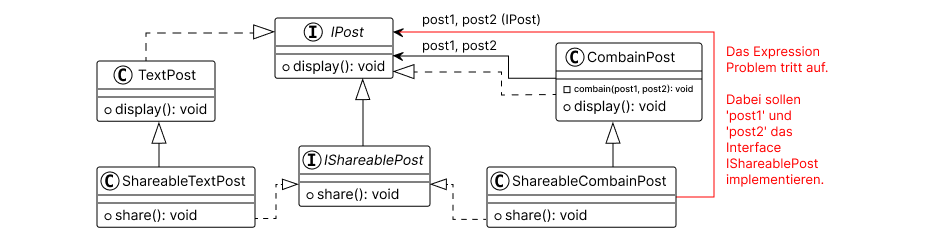
\includegraphics[width=0.98\textwidth]{Klassen-basiert.png}
        \caption{Klassen-basiert UML-Diagramm}
        \label{fig:KB}
      \end{center}
  \end{figure}

  \noindent Wie in Abbildung \ref{fig:KB} gezeigt, fügt die \texttt{share()}-Funktion hinzu, indem sie \texttt{IPost} erweitert. Probleme entstehen, wenn zusätzliche Funktionen wie \texttt{CombinePost} integriert werden sollen, da \texttt{post1} und \texttt{post2} ebenfalls das Interface \texttt{IShareablePost} implementieren müssen. Dies verdeutlicht das Expression Problem und erfordert Anpassungen am Code.

  \subsubsection*{Vorteile und Nachteile des klassenbasierten Ansatzes}


  Der klassenbasierte Ansatz zur Lösung des \textit{Expression Problems} ist leicht verständlich und fördert die Code-Wiederverwendung durch Vererbung \cite{gamma1994design}. Entwickler können bestehende Funktionalitäten einfach erweitern und wiederverwenden \cite{Cook1990}, was die Entwicklung und Wartung erleichtert \cite{torgersen2004expression}.

  Nachteile sind, dass Erweiterungen Änderungen in der Basisklasse erfordern und zu einer Neukompilierung führen \cite{wadler1998expression}. Neue Funktionen können den bestehenden Code beeinträchtigen und Anpassungen in allen abgeleiteten Klassen notwendig machen \cite{Reynolds1978}, was die Wartbarkeit erschwert und das Fehlerrisiko erhöht \cite{hughes1989functional}.
  


    \subsubsection{Visitor-Pattern}
    Das Visitor-Pattern ist ein Verhaltensmuster in der objektorientierten Programmierung, das die Trennung von Algorithmen und den Objektdatenstrukturen ermöglicht \cite{gamma1994design}. Es erlaubt das Hinzufügen neuer Operationen, indem eine Visitor-Klasse eingeführt wird, die die zu implementierenden Methoden für verschiedene Objekttypen definiert. Dieses Muster bewahrt die Integrität der ursprünglichen Klassen, indem es die Notwendigkeit vermeidet, deren Code zur Erweiterung von Funktionalitäten zu modifizieren \cite{gamma1994design}.\\
    
    \textbf{Im \hyperlink{beispiel1}{Beispiel 1}} der Social-Media App könnte das Visitor-Pattern verwendet werden, um unterschiedliche Funktionalitäten wie \textit{Display} und \textit{Shareable} zu implementieren, ohne die Post-Klassen selbst zu ändern. Dies wird durch die Einführung einer Visitor-Klasse erreicht, die spezifische Methoden für jede Art von Nachricht bereitstellt, sodass neue Operationen hinzugefügt werden können, ohne den bestehenden Code anzupassen.

    \begin{figure}[H]
      \begin{center}
        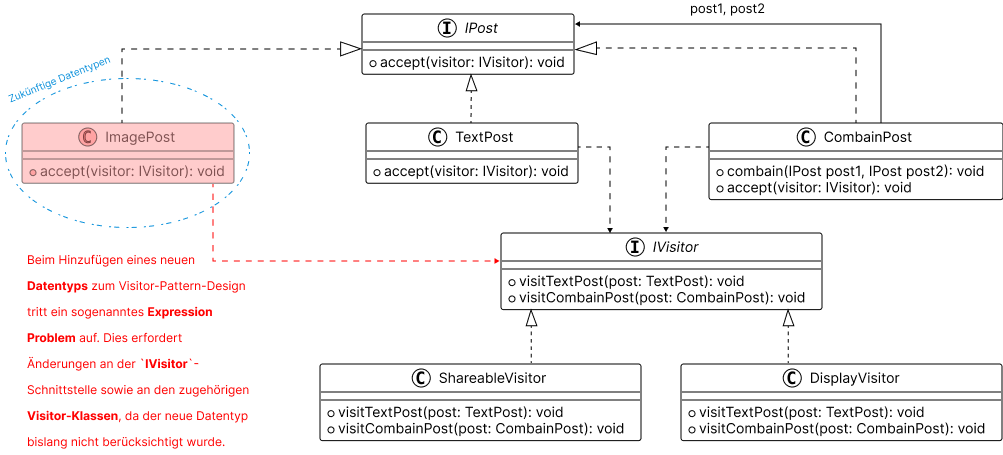
\includegraphics[width=0.97\textwidth]{Visitor-Pattern.png}
        \caption{Visitor-Pattern UML-Diagramm}
        \label{fig:VP}
      \end{center}
  \end{figure}

  \noindent Im UML-Diagramm Abbildung \ref{fig:VP} wird gezeigt, wie die Klassen \texttt{DisplayVisitor} und \texttt{ShareableVisitor} verschiedene Operationen auf \texttt{TextPost} und \texttt{CombinPost} anwenden. Das Visitor-Pattern ermöglicht neue Operationen, ohne die Post-Klassen zu ändern. Bei der Hinzufügung neuer Datentypen müssen jedoch auch die Visitor-Klassen aktualisiert werden, was das Expression Problem verdeutlicht und Codeanpassungen erfordert.


  \subsection*{Vorteile und Nachteile des Visitor-Patterns}

  Das Visitor-Pattern ermöglicht es, neue Operationen hinzuzufügen, ohne die bestehenden Klassen zu ändern, was die Flexibilität und Erweiterbarkeit des Codes erhöht \cite{gamma1994design}. Eine klare Trennung der Operationen von der Datenstruktur trägt dazu bei, den Code besser strukturiert und wartbarer zu halten \cite{Cook1990}. Dieses Designmuster bietet somit eine effiziente Möglichkeit, die Funktionalität eines Systems zu erweitern, ohne tiefgreifende Änderungen an den bestehenden Klassen vorzunehmen \cite{torgersen2004expression}.
  
  Jedoch kann das Visitor-Pattern zu komplexem und schwer wartbarem Code führen, insbesondere bei großen Objektstrukturen \cite{wadler1998expression}. Jede neue Klasse erfordert das Hinzufügen entsprechender Besuchermethoden, was den Entwicklungsaufwand erhöhen kann und die Übersichtlichkeit des Codes beeinträchtigt \cite{Reynolds1978}. Trotz dieser Herausforderungen bleibt das Visitor-Pattern ein wertvolles Werkzeug zur Strukturierung von komplexen Systemen und zur Trennung von Daten und Operationen \cite{hughes1989functional}.

\section{Generics und Programmiersprachenwahl}

\subsection{Einführung und Zweck von Generics}

Generics stellen ein grundlegendes Konzept der modernen Programmierung dar, welches die Definition von Typen als Parameter ermöglicht. Dadurch können Funktionen und Klassen so gestaltet werden, dass sie mit verschiedenen Datentypen arbeiten, ohne dass diese Datentypen explizit für jede Instanz spezifiziert werden müssen. Dies führt zu einer höheren Flexibilität und Wiederverwendbarkeit des Codes, da Algorithmen und Datenstrukturen unabhängig von konkreten Datentypen entwickelt werden können \cite{torgersen2004expression}.

Die Anwendung von Generics zielt darauf ab, die Typensicherheit und Lesbarkeit des Codes zu erhöhen. Die Kompilierungszeit-Überprüfung der Typen minimiert die Notwendigkeit von Typumwandlungen, wodurch die Wahrscheinlichkeit von Laufzeitfehlern reduziert wird und die Wartbarkeit des Codes verbessert wird \cite{hughes1989functional}.\\\\
Generics bieten zahlreiche Vorteile, wie:

\begin{itemize}
  \item \textbf{Typensicherheit}: Generics ermöglichen die Überprüfung der Typen zur Kompilierungszeit, was dazu beiträgt, Laufzeitfehler zu minimieren und die Zuverlässigkeit des Codes erheblich zu steigern \cite{wadler1998expression}.
  \item \textbf{Wiederverwendbarkeit}: Algorithmen und Datenstrukturen, die mit Generics geschrieben wurden, können mit verschiedenen Datentypen verwendet werden, ohne dass sie mehrfach implementiert werden müssen. Dies spart Zeit und Aufwand bei der Entwicklung \cite{torgersen2004expression}.
  \item \textbf{Lesbarkeit und Wartbarkeit}: Generics reduzieren die Notwendigkeit von Typumwandlungen und machen den Code dadurch einfacher zu lesen und zu verstehen. Dies fördert die Wartbarkeit und ermöglicht eine schnellere Fehlerbehebung \cite{wadler1998expression}.
\end{itemize}


  \subsection{Vorstellung der gewählten Programmiersprache}
  Die Wahl von TypeScript als Programmiersprache für die Implementierung der Lösungsansätze basiert auf meiner persönlichen Erfahrung sowie den umfassenden Möglichkeiten, die TypeScript für das Expression Problem bietet.\\

\textbf{Was ist TypeScript?}
  TypeScript ist eine von Microsoft entwickelte Open-Source-Programmiersprache, die als typisierte Obermenge von JavaScript fungiert und in reines JavaScript transpiliert. Die Sprache entstand aus ECMAScript, insbesondere nach bedeutenden Änderungen in der JavaScript-Programmierung durch die V8-Engine von Google. TypeScript bietet eine strenge Typisierung und unterstützt sowohl objektorientierte als auch imperative Programmierkonzepte. Es erweitert JavaScript um optionale statische Typen, Klassen, Module und Interfaces und stellt somit eine leistungsstarke Werkzeugkette für die Entwicklung großer JavaScript-Anwendungen dar \cite{typescript2019deepdive}.\\

\textbf{Gründe für die Wahl von TypeScript:} Es wurde aufgrund seiner starken Unterstützung für Generics ausgewählt, was die flexible und typsichere Implementierung von Lösungen für das Expression Problem ermöglicht \cite{torgersen2004expression}. Die statische Typisierung von TypeScript hilft, Fehler frühzeitig zu erkennen und sicherzustellen, dass Erweiterungen von Datentypen und Operationen korrekt typisiert sind \cite{rozentals2019typescript}. Zudem profitiert TypeScript von einer großen Entwicklergemeinschaft und einer Vielzahl an Bibliotheken, die kontinuierlich Lösungen für komplexe Probleme wie das Expression Problem bereitstellen \cite{typescript2019deepdive}.

\section{Datenzentrierter Ansatz mit Generics}
  \subsection{Beschreibung und Idee}
  Der datenzentrierte Ansatz adressiert das Expression Problem durch die Entwicklung eines Systems aus generischen Schnittstellen und Klassen, welches ohne Neukompilation bestehender Komponenten erweitert werden kann. Die Nutzung von Generics zur Definition abstrakter Datentypen, deren Spezifikation erst zur Laufzeit erfolgt, resultiert in einer sowohl flexiblen als auch zukunftssicheren Architektur. Die Integration neuer Datentypen und Funktionen ist ohne Beeinträchtigung existierender Strukturen möglich \cite{torgersen2004expression}. Die Entkopplung von Datenstrukturen und Algorithmen durch Generics steigert die Typensicherheit und ermöglicht eine flexiblere Datenhandhabung. Dies führt zu saubererem, wartbarerem und anpassungsfähigerem Code, der Änderungen am Datenmodell besser standhält \cite{wadler1998expression}.

  \subsection{Vorteile und Überwindung der Limitierungen des klassen-basierten Ansatzes}

  Die Vorteile des datenzentrierten Ansatzes resultieren direkt aus der Entkopplung von Daten und Algorithmen sowie der Nutzung von Generics zur Laufzeitspezifikation:

\begin{itemize}
    \item \textbf{Modularität und Erweiterbarkeit}: Neue Datentypen und Operationen lassen sich hinzufügen, ohne bestehende Klassen oder Methoden zu modifizieren, was die Anwendung modular und leicht erweiterbar macht \cite{torgersen2004expression}.
    \item \textbf{Vermeidung von Code-Duplizierung}: Generische Klassen und Methoden verringern die Notwendigkeit, ähnlichen Code für unterschiedliche Datentypen wiederholt zu schreiben, was die Wartbarkeit steigert und Fehlerquellen reduziert \cite{typescript2019deepdive}.
    \item \textbf{Typensicherheit}: Durch die Definition von Typen zur Compile-Zeit wird die Typensicherheit verbessert, wodurch viele Fehler frühzeitig erkannt und vermieden werden \cite{rozentals2019typescript}.
    \item \textbf{Wiederverwendbarkeit}: Die einfache Implementierung neuer generischer Klassen steigert die Flexibilität und Wiederverwendbarkeit des Codes, was die schnelle Anpassung an neue Anforderungen ermöglicht \cite{typescript2019deepdive}.
\end{itemize}

\subsection{Implementierung in TypeScript}

In diesem Abschnitt erläutern wir die Implementierung eines datenzentrierten Ansatzes in TypeScript. Dieser Ansatz zeigt, wie durch den Einsatz von Generics und dem CRTP\footnote{CRTP: Curiously Recurring Template Pattern} Design Pattern eine flexible und erweiterbare Struktur geschaffen werden kann, um das Ausdrucksproblem zu lösen.

Zunächst definieren wir die grundlegenden Interfaces und Klassen, um die Basisstruktur für verschiedene Post-Typen zu schaffen und erweitern diese dann, um zusätzliche Funktionalitäten hinzuzufügen.

\lstinputlisting[language=JavaScript, caption=Implementierung der \texttt{Post}| \texttt{TextPost} und \texttt{CombinePost} Klassen in TypeScript, label=lst:fixbounds]{codes/code1-2.ts}

\noindent \textbf{Erklärung:} Das Interface \texttt{IPost} definiert die \texttt{display()}-Methode für alle Posts. Die Klasse \texttt{TextPost} implementiert dieses Interface und ermöglicht die Anzeige von Text-Posts. \texttt{CombinePost} kombiniert zwei \texttt{IPost}-Instanzen und zeigt beide an.


Um die Funktionalität zum Teilen von Posts zu implementieren, fügen wir das Interface \texttt{Shareable} und zugehörige Klassen hinzu. Dies erlaubt es, Posts über Social-Media-Plattformen oder andere Kommunikationskanäle zu verbreiten.

\lstinputlisting[language=JavaScript, caption=Implementierung des \texttt{Shareable} Interfaces für teilbare Posts, label=lst:shareable]{codes/code3.ts}

\noindent \textbf{Erklärung:} Das Interface \texttt{IShareable} erweitert das \texttt{IPost}-Interface und fügt eine \texttt{share()}-Methode hinzu, die das Teilen von Inhalten ermöglicht. Die Klasse \texttt{ShareableTextPost} implementiert dieses Interface, indem sie von \texttt{TextPost} erbt, was das Teilen von Text-Posts ermöglicht. Ebenso erweitert die Klasse \texttt{ShareableCombinePost} die \texttt{CombinePost}-Klasse und implementiert das \texttt{IShareable}-Interface, wodurch kombinierte Posts geteilt werden können.\\

Um die Generizität festzulegen und instanziierbare Klassen zu schaffen, verwenden wir Fixpunktklassen. Diese Technik ist entscheidend für die Typsicherheit und Flexibilität der Architektur.

\lstinputlisting[language=JavaScript, caption=Definition von Fixpunktklassen zur Sicherstellung der Generizität, label=lst:fixbounds]{codes/code4.ts}

\noindent \textbf{Erklärung:} Das Interface \texttt{IShareablePostFix} setzt \texttt{IShareable} als Typparameter auf sich selbst fest, um die Typensicherheit und Konsistenz innerhalb des Typsystems zu gewährleisten. Dadurch wird sichergestellt, dass die Share-Funktionalität korrekt typisiert ist und keine Typfehler zur Laufzeit auftreten. Die Klassen \texttt{ShareableTextPostFix} und \texttt{ShareableCombinePostFix} spezifizieren die konkreten Typen für Text-Posts und kombinierte Posts, wodurch sie instanziierbar werden. Dies ermöglicht eine klare und präzise Verwendung der Typen in der Anwendung, was insbesondere bei der Erweiterung und Wartung des Codes von Vorteil ist.\\

Zum Abschluss demonstrieren wir die Nutzung der definierten Klassen, um die Funktionalität und Interoperabilität unseres Systems zu zeigen.

\lstinputlisting[language=JavaScript, caption=Beispielhafte Nutzung der implementierten Klassen, label=lst:usage]{codes/code5.ts}

Diese Implementierung zeigt, wie TypeScript genutzt werden kann, um ein flexibles und erweiterbares Typsystem zu schaffen. Der datenzentrierte Ansatz mit Generics ermöglicht eine Architektur, die sowohl Typensicherheit als auch Wiederverwendbarkeit gewährleistet. Neue Post-Typen und Methoden können hinzugefügt werden, ohne den bestehenden Code wesentlich verändern zu müssen, was den Kern des Ausdrucksproblems darstellt.\footnote{Der gesamte gezeigte Code ist auf der GitHub-Seite verfügbar. Siehe: \url{https://github.com/artamrj/ExpressionProblemRevisited/tree/main/CODE}.}

\section{Operationszentrierter Ansatz mit Generics}


\subsection{Konzept und Erklärung}

Der operationszentrierte Ansatz nutzt Generics, um eine klare Trennung zwischen Datenstrukturen und den darauf anwendbaren Operationen zu schaffen. Generische Schnittstellen definieren Operationen wie Posten, Teilen und Validieren, die auf verschiedene Datentypen anwendbar sind. Neue Operationen können hinzugefügt werden, ohne bestehende Datenstrukturen zu ändern, was die Modularität und Wiederverwendbarkeit des Codes fördert \cite{torgersen2004expression}. Zusätzlich erhöhen Generics die Typsicherheit und verbessern die Wartbarkeit des Systems \cite{rozentals2019typescript}.

Im Kern liegt dieser Ansatz in der Erweiterung des Visitor-Patterns. Neue Datentypen oder Operationen können hinzugefügt werden, ohne bestehende Datenstrukturen zu modifizieren. Generics ermöglichen eine flexible und erweiterbare Architektur, indem sie in die Definition der Besucher und der zu besuchenden Elemente integriert werden \cite{wadler1998expression}.

\subsection{Anwendung von Generics im Visitor-Pattern}

Im operationszentrierten Ansatz mit Generics werden generische Typen in den Visitor-Schnittstellen und den besuchten Elementen verwendet. Dies ermöglicht es Besuchern, spezifische Methoden für neue Datentypen zu implementieren, ohne die bestehenden Klassen zu verändern \cite{hughes1989functional}. In \hyperlink{beispiel1}{Beispiel 1} könnte das Hinzufügen einer neuen Funktion für Shareable-Posts durch die Erweiterung der Visitor-Schnittstellen erfolgen, sodass diese neue Funktion ohne Änderungen an den bestehenden Text-, Bild- oder Video-Beiträgen integriert werden kann.

\subsection{Vorteile und Nachteile}

Der operationszentrierte Ansatz mit Generics ermöglicht das Hinzufügen neuer Operationen ohne Änderungen am bestehenden Code, was die Erweiterbarkeit und Anpassungsfähigkeit des Systems fördert \cite{rozentals2019typescript}. Die Trennung von Operationen und Daten verbessert die Modularität und Wartbarkeit des Codes \cite{hughes1989functional}. Generics erhöhen die Typensicherheit durch Typüberprüfung zur Compile-Zeit und reduzieren potenzielle Laufzeitfehler \cite{typescript2019deepdive}.

Dieser Ansatz bringt jedoch eine erhöhte Komplexität bei der Implementierung und dem Verständnis des Codes mit sich, besonders für Entwickler mit weniger Erfahrung in Generics. Die korrekte Anwendung von Generics im Visitor-Pattern erfordert mehr Fachwissen und kann die Einarbeitungszeit verlängern \cite{Krishnamurthi1998}.


\section{Schluss}
  \subsection{Zusammenfassung}

  In dieser Ausarbeitung wurde das Expression Problem von seinen historischen Wurzeln bis zu modernen Lösungen mit Generics in TypeScript untersucht. Zu Beginn wurden die Arbeiten von John Reynolds \cite{Reynolds1978} und die Definition von Philip Wadler \cite{wadler1998expression} erläutert, um die Herausforderung der Erweiterbarkeit von Datentypen und Operationen ohne Neukompilierung des Codes zu verdeutlichen.
  
  Klassische Ansätze wie der klassenbasierte Ansatz und das Visitor-Pattern wurden vorgestellt \cite{gamma1994design}, gefolgt von einer Analyse der Vorteile von Generics für Typensicherheit und Wiederverwendbarkeit \cite{rozentals2019typescript}. Es wurde gezeigt, wie TypeScript aufgrund seiner starken Unterstützung für Generics ausgewählt wurde \cite{typescript2019deepdive}. Der datenzentrierte Ansatz ermöglicht eine flexible und erweiterbare Architektur, während der operationszentrierte Ansatz die Modularität verbessert \cite{torgersen2004expression}. Insgesamt bietet TypeScript mit Generics effektive Lösungen für das Expression Problem, indem Flexibilität und Typensicherheit vereint werden.


  \subsection{Fazit}

  Die Analyse des \textit{Expression Problems} und die Implementierung der Lösungen mit Generics in TypeScript haben gezeigt, dass diese Ansätze entscheidende Vorteile bieten. Generics ermöglichen die Entwicklung flexibler und typsicherer Software, die sowohl modular als auch wartbar ist. TypeScript hat sich als geeignete Sprache erwiesen, um diese Konzepte effektiv umzusetzen.
  
  Die vorgestellten Ansätze zur Lösung des \textit{Expression Problems} zeigen, dass durch den Einsatz von Generics die Erweiterbarkeit und Wiederverwendbarkeit von Code erheblich verbessert werden können. Diese Techniken bieten eine robuste Grundlage für die Entwicklung zukünftiger Softwareprojekte. Nachteile wie erhöhte Komplexität bei der Implementierung können durch sorgfältige Planung und Design minimiert werden.
  
  Insgesamt bieten die Lösungen für das \textit{Expression Problem} wertvolle Ansätze für die Softwareentwicklung und tragen zur Schaffung von zukunftssicheren Anwendungen bei.
  
 \newpage
\label{sect:bib}
\bibliographystyle{plain}
%\bibliographystyle{alpha}
%\bibliographystyle{unsrt}
%\bibliographystyle{abbrv}
\bibliography{literatur}

\end{document}

